%====================================================================================================
% ?????
%====================================================================================================
% TCC
%----------------------------------------------------------------------------------------------------
% Autor				: Jasane Schio
% Orientador		: Gedson Faria
% Co-Orientador		: Angelo Darcy
% Instituição 		: UFMS - Universidade Federal do Mato Grosso do Sul
% Departamento		: CPCX - Sistema de Informação
%----------------------------------------------------------------------------------------------------
% Data de criação	: 01 de Outubro de 2015
%====================================================================================================
% NO FUTURO
\chapter{Resultados} 

Para a execução dos tipos de testes, o campo foi dividido verticalmente em cinco partes, de vinte e nove centimetros cada, e horizontalmente em três parte de quarenta e um centimetro cada, somando um total de quinze areas de calibração, nomeadas alfabeticamente de A à O, como mostrado na Figura \ref{campodivisao}.

\begin{figure}[!: h]
		\centering
		\includegraphics[width=0.3\textwidth]{campodivisao.pdf}
		\caption{Divisao do campo em quinze partes nomeadas alfabeticamente.}
		\label{campodivisao}
	\end{figure}
	
Em cada areas de calbração estão dispostas cinco cores: Vermelho  e Verde na primeira linha, Amarelo, Azul e Laranja na segunda. As cores estão distantes verticalmente \textit{7.5cm}, na primeria linha a distancia entre as cores é  de \textit{11 cm} e na segunda linha de \textit{7.2 cm}. Um  melhor detalhamento da disposiçao das cores é  mostrado na Figura \ref{disposicaoparte}. No total estavam disposto no campo quinze pontos de cada cor.

\begin{figure}[!: h]
		\centering
		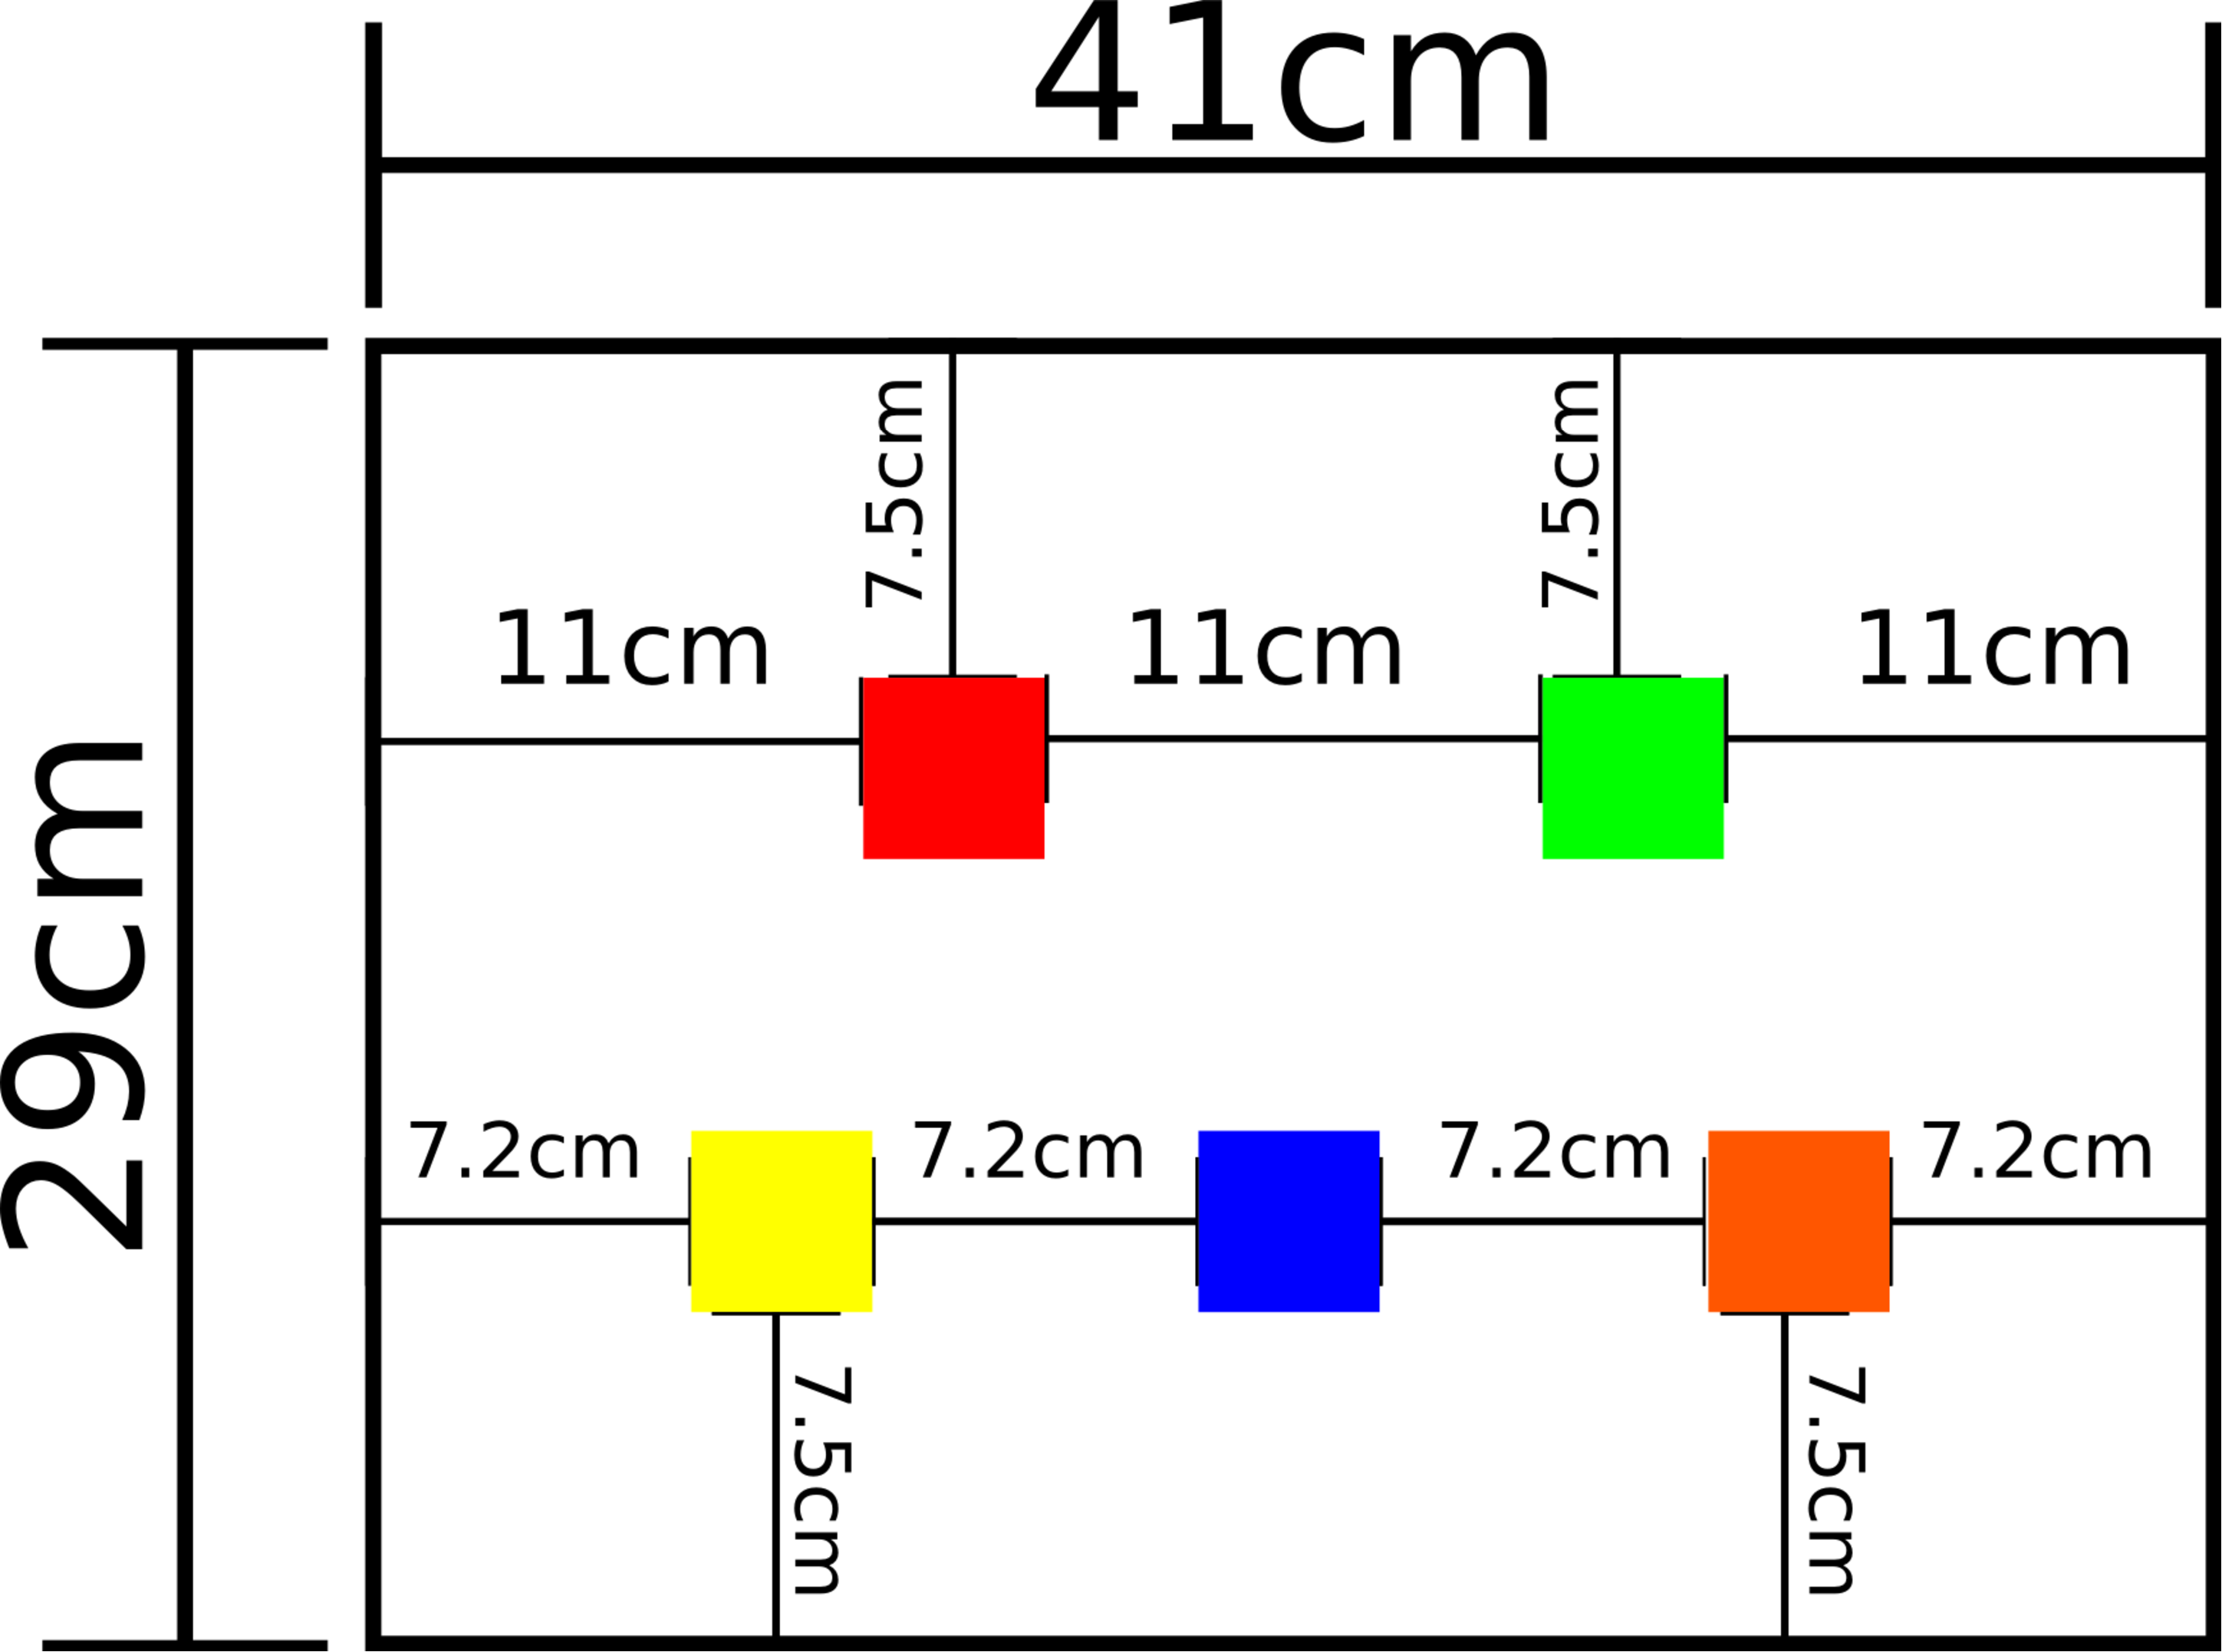
\includegraphics[width=0.3\textwidth]{disposicaoparte.pdf}
		\caption{Disposição dos objetos coloridos dentro de cada uma das partes}
		\label{disposicaoparte}
	\end{figure}
	\newpage
\section{Teste Geral}
Este foi o teste feito com o campo inteiro, usando todas as quinze partes. Três variaveis fora usadas para este teste, foram elas \textit{Brilho}, \textit{Contraste} e  \textit{Limiar}, este ultimo ajustava a sensibilidade da deteção de borda do algoritmo de Canny. Os valores a serem usados para cada variarel estao deisposto na tabela a baixo:

\begin{table}[h]
\centering
\caption{Tabela de Testes}
\begin{tabular}{r|c|l}
Brilho & Constrate & Limiar \\ % Note a separação de col. e a quebra de linhas
\hline                               % para uma linha horizontal
0 & 30 &  20\\
\hline 
20 &  44 &  40\\
\hline 
40 & 58 &  60 \\
\hline 
60 &  72 &  80\\
\hline 
80 & 86  & 100\\
\hline 
100 & 100  & \\
\hline  
\end{tabular}
\end{table}
Note que o valor de contraste iniciando em 30, pois verificou-se que abaixo disso a imagem fica totalmente da escura, sendo assim é inviavel o teste com essa configuração. Ja o valor de limiar inicia em 20 pois verificou-se que um valor de limiar menor que 20 possuiu muito ruido e detecçoes de pequenas linhas, como luzes e sombras, sendo assim tambem inviavel.
O total de testes executados com o campo todo foi:
\begin{displaymath}
 Contraste \times Brilho \times Limiar \equiv 6 \times 6 \times 4 = 180
\end{displaymath}
	
	
	
	
	
%	\begin{figure}
%\centering
%\begin{subfigure}{.5\textwidth}
%  \centering
%  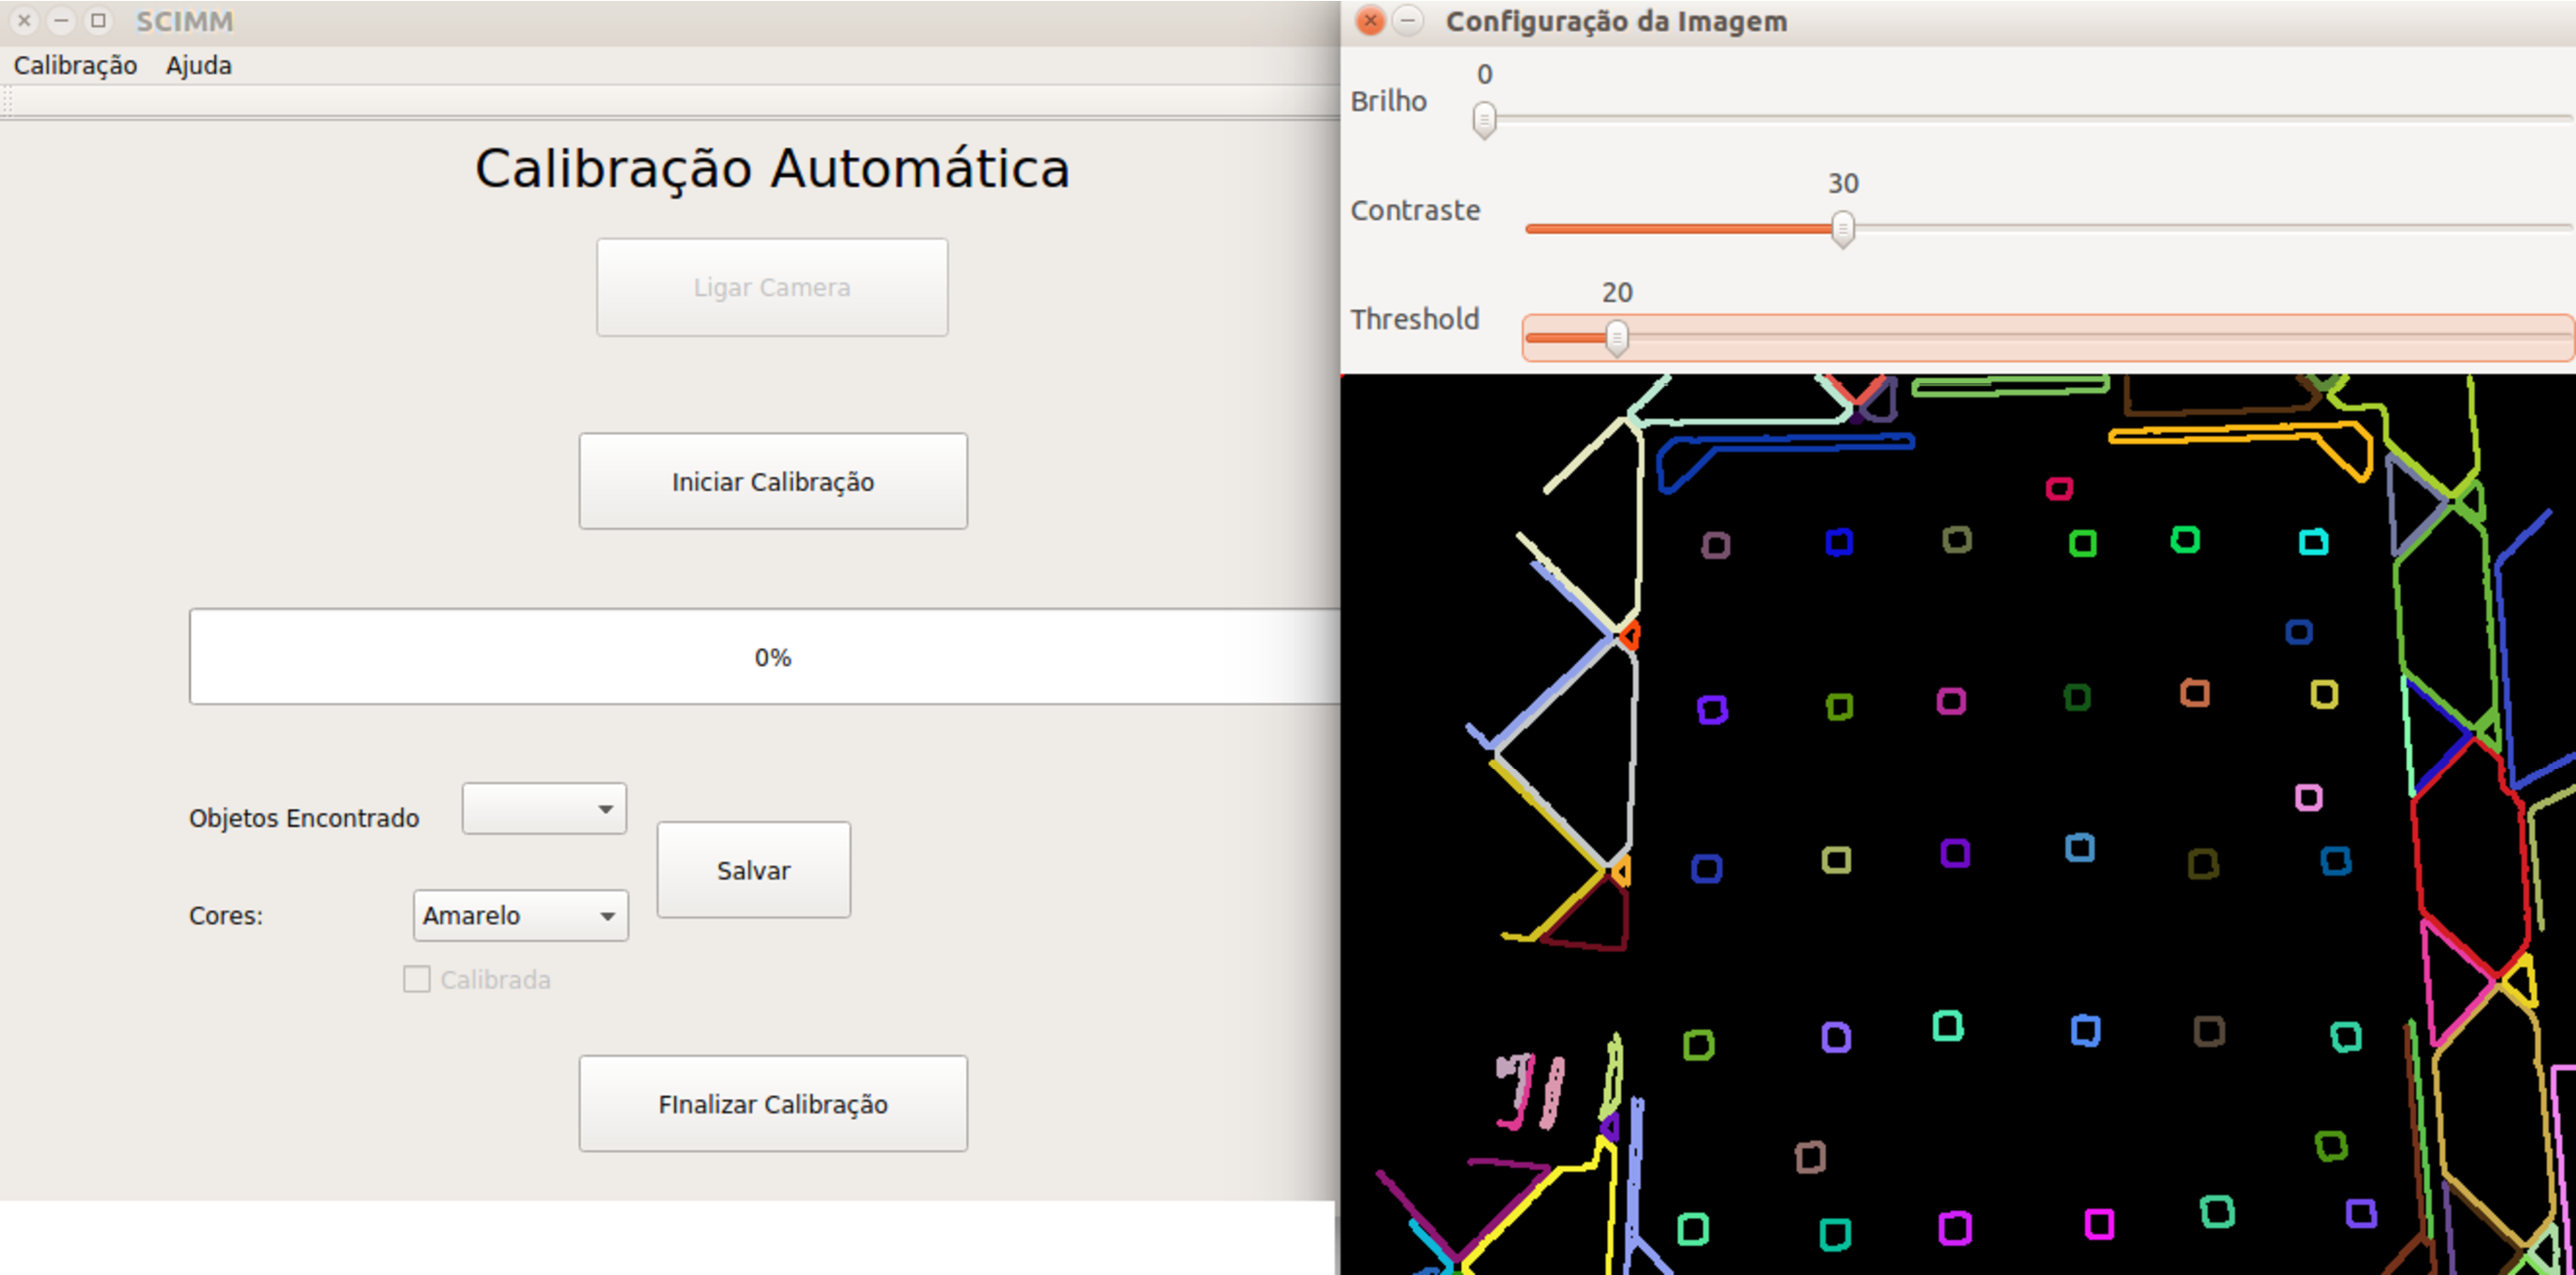
\includegraphics[width=.9\linewidth]{exgeral1.pdf}
%  \caption{Configuraçao de Imagem antes da calibracao}
%  \label{fig:sub1}
%\end{subfigure}%
%\begin{subfigure}{.5\textwidth}
%  \centering
%  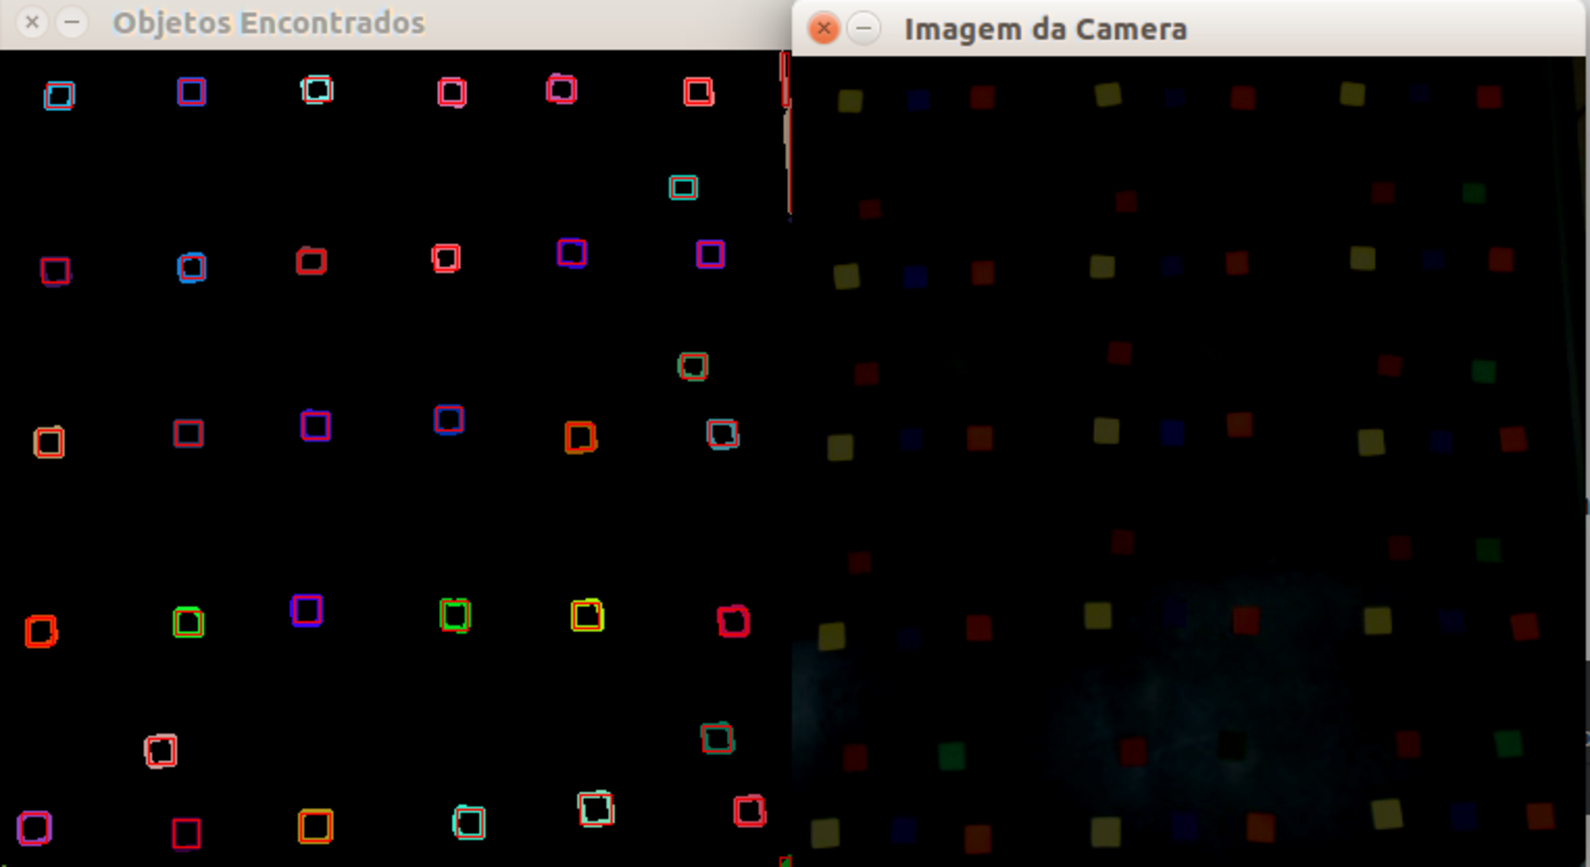
\includegraphics[width=.9\linewidth]{exgeral2.pdf}
%  \caption{Resultado final da configuracao mostrada antes de se iniciar a calibracao}
%  \label{fig:sub2}
%\end{subfigure}
%\caption{•}
%\label{fig:test}
%\end{figure}

Em cada um dos 180 testes foram analisadas 11 variaveis, sendo elas:
\begin{description}
\item [Q-E] significando a quantidade de objetos, gerais, detectado pela deteccao de contornos;
\item[OC-E] significando a quantidade de objetos-cor encontrados durante a analise da imagem; 
\item[C-E] significando a quantidade de objetos-cor encontrados que realmente correspondiam aos objetos-cor desejados;
\item[\%] significando a porcentagem de \textbf[C-E] relativo a \textbf[OC-E];
\item[AZUL] significando a quantidade de objetos encontrado no melhor caso obtido;
\item[AMARELO] significando a quantidade de objetos encontrado no melhor caso obtido;
\item[LARANJA] significando a quantidade de objetos encontrado no melhor caso obtido;
\item[VERDE] significando a quantidade de objetos encontrado no melhor caso obtido;
\item[VERMELHO] significando a quantidade de objetos encontrado no melhor caso obtido;
\item[T-E] significando o total de cores que foram encontrados;
\item[P-E] significando o total de cores que foram encontrados corretamente, ou seja todas as quinze partes da cor disposta em campo;
\end{description}
	
	
	
	
	Em uma analise inicial sobre o \textbf{Teste Geral} foi encontrado, o considerado, limiar otimo para detecçao, sendo este aquele que em \textbf{P-E} de todas as cores obtiveram as melhores porcentagem de \textbf{\%}, como mostra a Figura \ref{graficoanaliselimiar}. 
	
	
	
	
	Mesmo sabendo que o limiar com maior sensibilidade é o limiar 20, o mesmo nao obteve um desenpenho tao continuo em \textbf{\%} quanto o limiar 40.
	
	\begin{figure}[!: h]
		\centering
		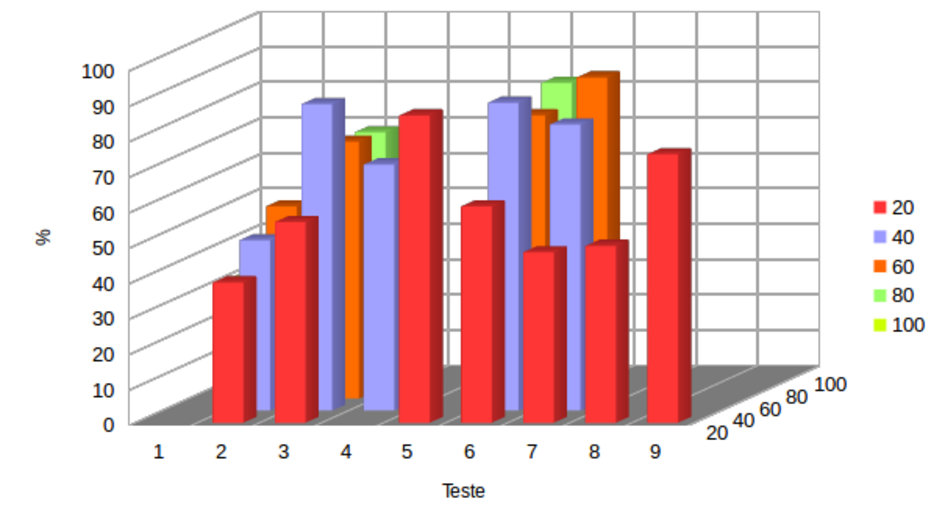
\includegraphics[width=0.8\textwidth]{testegeralgraficolimiar.pdf}
		\caption{Grafico de limiar de acordo com a porcentagem de objetos-cor encontrados.}
		\label{graficoanaliselimiar}
	\end{figure}
	
	\section{Teste Por Area}
	Ao final dos testes geral identificamos o limiar com maior ocorrencia de ojetos detectados com precisao. Para diminuir a quantidade de casos de teste por area que  ateriormente seria:
	\begin{displaymath}
 Contraste \times Brilho \times Limiar \times Areas \equiv 6 \times 6 \times 4  \times 15 = 2160
\end{displaymath}

Optou-se entao a usar o limiar 40, assim a quantidade de testes diminuiu drasticamente para apenas um quarto do valor original.
	\begin{displaymath}
 Contraste \times Brilho \times Limiar \equiv 6 \times 6 \times 15 = 540
\end{displaymath}